\documentclass[11pt]{article}
 
\usepackage[text={6in,8.1in},centering]{geometry}
 
\usepackage{enumerate}
\usepackage{amsmath,amsthm,amssymb}
 
\usepackage{pstricks}
\usepackage{pst-solides3d}
\usepackage{pstricks-add}
\usepackage{graphicx}
\usepackage{pst-tree}
\usepackage{pst-poly}
\usepackage{calc,ifthen}
\usepackage{float}
\usepackage{multicol}
\usepackage{multirow}
\usepackage{array}
\usepackage{longtable}
\usepackage{tikz}
\usepackage{tkz-berge}
\usepackage{fancyhdr}
 
 
 
\newtheorem{proposition}{Proposition}
\newtheorem{theorem}{Theorem}
\newtheorem{lemma}{Lemma}
\newtheorem{corollary}{Corollary}
 
\theoremstyle{definition}
\newtheorem{definition}{Definition}
 
\title{This is our Title\footnote{Supported in part by National Science Foundation (NSF).}}
\author{Jordan Blocher\thanks{Department of Mathematics, University of Nevada-Reno, Reno, TX, USA. jordanblocher@gmail.com.} \and Samantha Hampton\thanks{Department of Mathematics, University of Arkansas, Fayetteville, AR, USA}\and Christopher Linden\thanks{University of California Los Angeles, Los Angeles, CA,USA }}
\date{\today}
 
 
\def\R{\mbox{$\mathbb R$}}
\def\Q{\mbox{$\mathbb Q$}}
\def\Z{\mbox{$\mathbb Z$}}
\def\N{\mbox{$\mathbb N$}}
\def\C{\mbox{$\mathbb C$}}
\def\Sym{\operatorname{Sym}}
\def\lcm{\operatorname{lcm}}
\def\adj{\operatorname{adj}}
\def\inc{\operatorname{inc}}
\def\Cay{\operatorname{Cay}}
\def\Geom{\operatorname{\cal G}}
\def\ker{\operatorname{ker}}
\def\kernel{\operatorname{ker}}
\def\automorphism{\operatorname{Aut}}
\def\endomorphism{\operatorname{End}}
\def\inner{\operatorname{Inn}}
\def\outer{\operatorname{Out}}
\def\crossing{\operatorname{cr}}
\def\cent{\textcent}
 
\renewcommand{\emptyset}{\O}
 
 
\newcounter{ZZZ}
\newcounter{XXX}
\newcounter{XX}
 
\headsep25pt\headheight20pt
 
 
\pagestyle{fancyplain}
\lhead{\fancyplain{}{\small\bfseries Authors,\ \ This is our Title}}
\rhead{\fancyplain{}{\small\bfseries\thepage}}
\cfoot{\ \hfill\tiny\sl Draft printed on \today}
 
 
\setlength{\extrarowheight}{2.5pt} % defines the extra space in tables
 
 
 
\begin{document}
 
\maketitle
\begin{center}
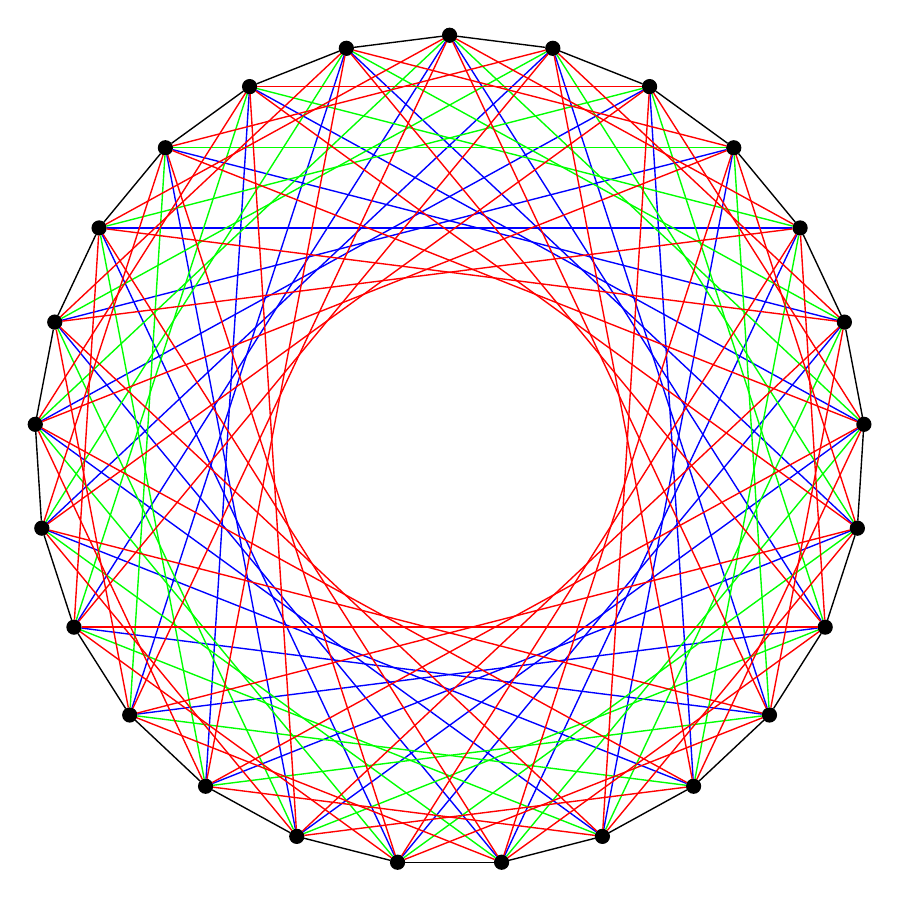
\begin{tikzpicture}


\GraphInit[vstyle=Simple]
\tikzset{VertexStyle/.append style = {minimum size = 5pt, inner sep = 0pt}}

\Vertex[x=187.5pt,y=337.5pt]{0};
\Vertex[x=224.80348307472823pt,y=332.7874741692947pt]{1};
\Vertex[x=259.7630511152573pt,y=318.94600200657953pt]{2};
\Vertex[x=290.1820658893033pt,y=296.8452941132117pt]{3};
\Vertex[x=314.14918882530225pt,y=267.87401924684946pt]{4};
\Vertex[x=330.15847744427305pt,y=233.85254915624213pt]{5};
\Vertex[x=337.2040092642407pt,y=196.91857792939703pt]{6};
\Vertex[x=334.8430876093033pt,y=159.3928028121413pt]{7};
\Vertex[x=323.22405786990294pt,y=123.63310626523908pt]{8};
\Vertex[x=303.0769864163684pt,y=91.88640153769651pt]{9};
\Vertex[x=275.667787843871pt,y=66.14745084375791pt]{10};
\Vertex[x=242.71868290270174pt,y=48.0335271167623pt]{11};
\Vertex[x=206.2999850346457pt,y=38.682794802828326pt]{12};
\Vertex[x=168.70001496535434pt,y=38.682794802828326pt]{13};
\Vertex[x=132.2813170972983pt,y=48.03352711676226pt]{14};
\Vertex[x=99.3322121561291pt,y=66.14745084375782pt]{15};
\Vertex[x=71.92301358363159pt,y=91.88640153769656pt]{16};
\Vertex[x=51.77594213009703pt,y=123.63310626523916pt]{17};
\Vertex[x=40.1569123906967pt,y=159.3928028121413pt]{18};
\Vertex[x=37.795990735759275pt,y=196.91857792939695pt]{19};
\Vertex[x=44.841522555726954pt,y=233.8525491562421pt]{20};
\Vertex[x=60.85081117469775pt,y=267.8740192468495pt]{21};
\Vertex[x=84.81793411069665pt,y=296.8452941132117pt]{22};
\Vertex[x=115.23694888474257pt,y=318.9460020065795pt]{23};
\Vertex[x=150.1965169252717pt,y=332.7874741692946pt]{24};

\SetUpEdge[lw         = .5pt,
            color      = black,
            labelcolor = black]

\Edge(24)(0)
\Edge(0)(1)
\Edge(1)(2)
\Edge(2)(3)
\Edge(3)(4)
\Edge(4)(5)
\Edge(5)(6)
\Edge(6)(7)
\Edge(7)(8)
\Edge(8)(9)
\Edge(9)(10)
\Edge(10)(11)
\Edge(11)(12)
\Edge(12)(13)
\Edge(13)(14)
\Edge(14)(15)
\Edge(15)(16)
\Edge(16)(17)
\Edge(17)(18)
\Edge(18)(19)
\Edge(19)(20)
\Edge(20)(21)
\Edge(21)(22)
\Edge(22)(23)
\Edge(23)(24)

\SetUpEdge[lw         = .5pt,
            color      = blue,
            labelcolor = black]

\Edge(0)(8)
\Edge(2)(10)
\Edge(4)(12)
\Edge(6)(14)
\Edge(8)(16)
\Edge(10)(18)
\Edge(12)(20)
\Edge(14)(22)
\Edge(16)(24)
\Edge(18)(1)
\Edge(20)(3)
\Edge(22)(5)
\Edge(24)(7)
\Edge(1)(9)
\Edge(3)(11)
\Edge(5)(13)
\Edge(7)(15)
\Edge(9)(17)
\Edge(11)(19)
\Edge(13)(21)
\Edge(15)(23)
\Edge(17)(0)
\Edge(19)(2)
\Edge(21)(4)
\Edge(23)(6)

\SetUpEdge[lw         = .5pt,
            color      = green,
            labelcolor = black]

\Edge(0)(6)
\Edge(6)(12)
\Edge(12)(18)
\Edge(18)(24)
\Edge(24)(5)
\Edge(5)(11)
\Edge(11)(17)
\Edge(17)(23)
\Edge(23)(4)
\Edge(4)(10)
\Edge(10)(16)
\Edge(16)(22)
\Edge(22)(3)
\Edge(3)(9)
\Edge(9)(15)
\Edge(15)(21)
\Edge(21)(2)
\Edge(2)(8)
\Edge(8)(14)
\Edge(14)(20)
\Edge(20)(1)
\Edge(1)(7)
\Edge(7)(13)
\Edge(13)(19)
\Edge(19)(0)

\SetUpEdge[lw         = .5pt,
            color      = red,
            labelcolor = black]

\Edge(0)(4)
\Edge(4)(8)
\Edge(8)(12)
\Edge(12)(16)
\Edge(16)(20)
\Edge(20)(24)
\Edge(24)(3)
\Edge(3)(7)
\Edge(7)(11)
\Edge(11)(15)
\Edge(15)(19)
\Edge(19)(23)
\Edge(23)(2)
\Edge(2)(6)
\Edge(6)(10)
\Edge(10)(14)
\Edge(14)(18)
\Edge(18)(22)
\Edge(22)(1)
\Edge(1)(5)
\Edge(5)(9)
\Edge(9)(13)
\Edge(13)(17)
\Edge(17)(21)
\Edge(21)(0)
\Edge(0)(9)
\Edge(9)(18)
\Edge(18)(2)
\Edge(2)(11)
\Edge(11)(20)
\Edge(20)(4)
\Edge(4)(13)
\Edge(13)(22)
\Edge(22)(6)
\Edge(6)(15)
\Edge(15)(24)
\Edge(24)(8)
\Edge(8)(17)
\Edge(17)(1)
\Edge(1)(10)
\Edge(10)(19)
\Edge(19)(3)
\Edge(3)(12)
\Edge(12)(21)
\Edge(21)(5)
\Edge(5)(14)
\Edge(14)(23)
\Edge(23)(7)
\Edge(7)(16)
\Edge(16)(0)

\end{tikzpicture}
\end{center}
 
$\\$
$\\$
$\\$

\begin{abstract}
This is our abstract. We are going to have much more text than this in here. This is our abstract. We are going to have much more text than this in here. This is our abstract. We are going to have much more text than this in here. This is our abstract. We are going to have much more text than this in here. This is our abstract. We are going to have much more text than this in here. This is our abstract. We are going to have much more text than this in here. This is our abstract. We are going to have much more text than this in here. 
\end{abstract}
 
\section{Introduction}
 
Let $\Gamma$ be a finite group with a subset A. The \emph{Cayley digraph}, denoted Cay($\Gamma$,A), is a digraph with vertex set $\Gamma$, such that (x,y) is a directed edge if and only if $yx^{-1}$ $\in$ A.
In this paper we will be working with $\mathbb{Z}_m$ as our vertex set, and will denote these Cayley graphs as Cay(m,A).
 

 \begin{figure}[h]
\begin{center}

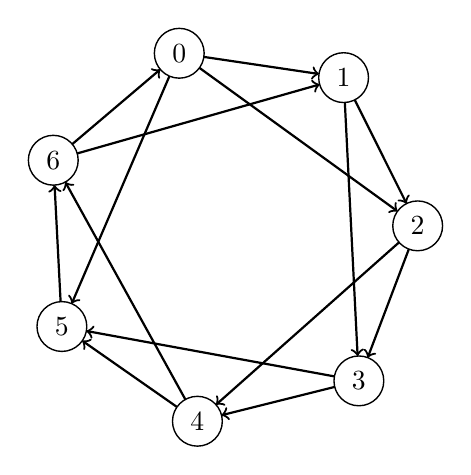
\begin{tikzpicture}


\Vertex[x=170.0508492385226pt,y=257.44793707070056pt]{0};
\Vertex[x=229.43059777036808pt,y=248.64351388167475pt]{1};
\Vertex[x=256.19943380501326pt,y=195.0860839875888pt]{2};
\Vertex[x=234.95343715746685pt,y=139.06822600729095pt]{3};
\Vertex[x=176.6059109911555pt,y=124.48269654626677pt]{4};
\Vertex[x=127.63862734371301pt,y=158.71121570275264pt]{5};
\Vertex[x=124.5266485799639pt,y=218.79228696858095pt]{6};
\tikzset{EdgeStyle/.style={->}}
\Edge(1)(2)
\Edge(0)(1)
\Edge(6)(0)
\Edge(5)(6)
\Edge(4)(5)
\Edge(3)(4)
\Edge(2)(3)
\Edge(0)(2)
\Edge(2)(4)
\Edge(4)(6)
\Edge(6)(1)
\Edge(1)(3)
\Edge(3)(5)
\Edge(0)(5)
\end{tikzpicture}
\end{center}
\caption{ Cay($\mathbb{Z}_7$, \{1,2\}).}
\end{figure}
 
An important property of Cayley digraphs is the Cayley digraph Cay(m,A) is vertex-symmetric. This property allows us to define extremal functions for these digraphs. 
For any positive integer $d$ we define
\[
m(d,A) =\ max\{m | d(m,A) \leq d\},
\]
the largest positive integer $m$ such that the diameter, d(m,A), of the Cayley digraph Cay(m,A) is less than or equal to d. For positive integers $d$ and $k$,
\[ 1) = d+1\text{, and}
\]
\[
m(d,2) = \lfloor \frac{d(d+4)}{3} \rfloor +\text{1 for $d$} \geq 2.
\]
 
In this paper we will examine the case when k = 3. The current bounds for this case is
\[
\frac{176}{2197}d^3 + O(d^2) \leq m(d,3) \leq \frac{1}{14-3\sqrt{3}}(d+3)^3 .
\]
 
 
\end {document}